\section{Transformaciones de features}
\label{sec:transformaciones}

El análisis distribucional presentado en la Sección~\ref{sec:analisis_distribucional} 
mostró que varias features presentan distribuciones sesgadas a la derecha. Con el objetivo de evaluar si una representación más simétrica de 
estas variables mejora su capacidad predictiva sobre la señal EEG, se 
exploraron dos transformaciones. La primera es el logaritmo natural:
%
\begin{equation}
    f(x) = \log(x)
\end{equation}
%
cuya aplicación se justifica para features con distribuciones de cola 
larga, ya que contrae los valores extremos y reduce el sesgo a la derecha. 
La segunda es la transformación logit:
%
\begin{equation}
    f(x) = \log\left(\frac{x}{1-x}\right)
\end{equation}
%
que se aplica a variables acotadas en el intervalo $(0,1)$, llevándolas 
al espacio real $(-\infty, +\infty)$, lo cual es teóricamente más apropiado 
para su uso como predictor en un modelo lineal.

Las transformaciones exploradas para cada feature se resumen en la 
Tabla~\ref{tab:transformaciones}. La elección de cada transformación 
estuvo guiada por las características distribucionales observadas en 
la Sección~\ref{sec:analisis_distribucional}. A continuación se detalla 
el análisis particular de cada feature.

\begin{table}[H]
\centering
\label{tab:transformaciones}
\begin{tabular}{p{3.5cm}p{4.5cm}p{4.5cm}}
\toprule
\textbf{Categoría} & \textbf{Feature} & \textbf{Transformaciones} \\
\midrule
\multirow{2}{*}{Bottom-up} 
  & \feat{saliencia\_pixel}      & $\log(x)$ \\
  & \feat{saliencia\_media}      & $\log(x)$ \\
\midrule
\multirow{2}{*}{Similitud con el target} 
  & \feat{similitud\_pixel}      & $\log(x)$ \\
  & \feat{similitud\_media}      & $\log(x)$ \\
\midrule
\multirow{2}{*}{\parbox{3.5cm}{Estado interno del\\proceso bayesiano}} 
  & \feat{ganancia\_informacion} & $\log(x)$ \\
  & \feat{posterior}             & $\log(x)$, logit$(x)$ \\
\midrule
\multirow{2}{*}{Calidad de la decisión} 
  & \feat{gap\_entropia}         & $\log(x)$ \\
  & \feat{distancia\_grilla}     & $\log(x)$ \\
\midrule
\multirow{2}{*}{\parbox{3.5cm}{Competencia entre\\candidatos}}
  & \feat{competencia\_densidad} & $\log(x)$ \\
  & \feat{competencia\_fp\_max}  & $\log(x)$ \\
\bottomrule
\end{tabular}
\caption{Transformaciones exploradas por feature.}
\end{table}

\subsubsection{Transformaciones a features Bottom-Up}

Las features \feat{saliencia\_media} y \feat{saliencia\_pixel} presentan 
distribuciones fuertemente sesgadas a la derecha en su escala original, 
con la mayor parte de los valores concentrados cerca de cero y una cola 
larga hacia valores altos. La aplicación de $\log(x)$ redujo el sesgo 
en ambos casos. En \feat{saliencia\_media}, la distribución resultante 
es aproximadamente simétrica y unimodal. 

\begin{figure}[H]
    \centering
    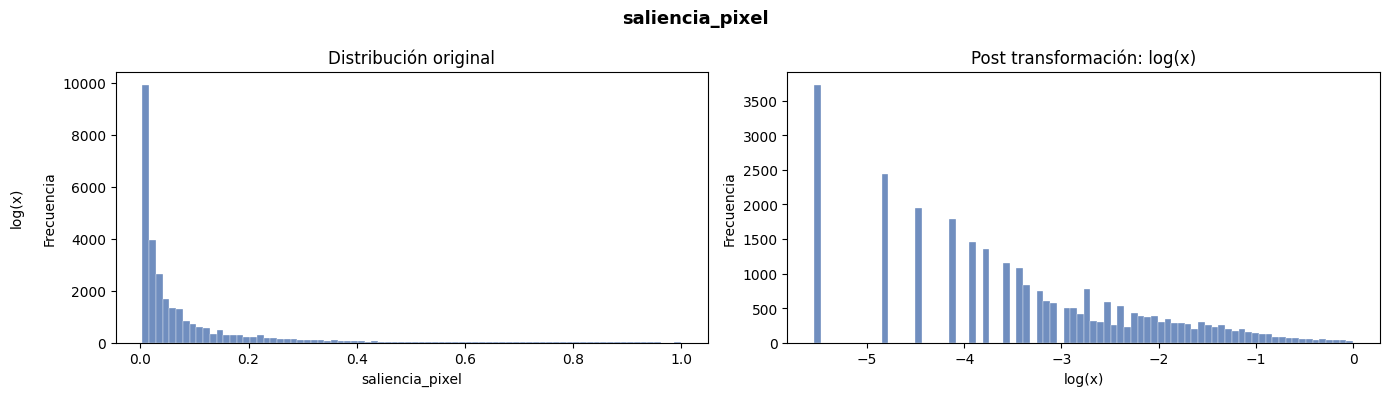
\includegraphics[width=\textwidth]{chapters/03_analisis_features/images/transf_saliencia_pixel}
    \caption{Distribución de la variable saliencia\_pixel transformada}
    \label{fig:transf_saliencia_pixel}
\end{figure}

En \feat{saliencia\_pixel}, 
la transformación también reduce el sesgo, aunque la distribución 
resultante presenta una estructura multimodal con picos discretos, 
lo cual es consistente con la naturaleza puntual de esta feature: 
a diferencia de \feat{saliencia\_media}, que promedia la saliencia 
sobre una celda completa, \feat{saliencia\_pixel} toma el valor en 
el píxel exacto de fijación, lo que introduce mayor variabilidad 
y concentración en valores específicos.

\begin{figure}[H]
    \centering
    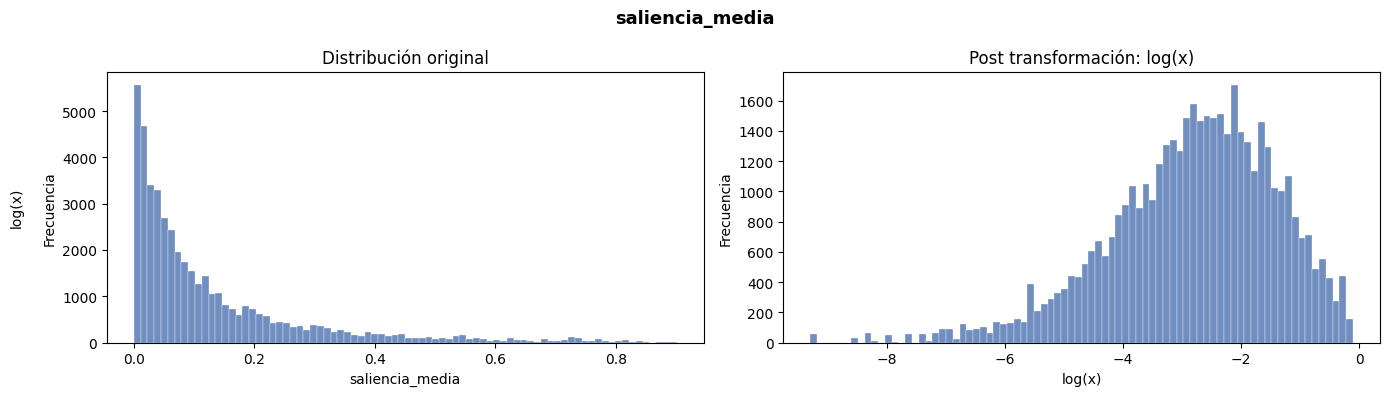
\includegraphics[width=\textwidth]{chapters/03_analisis_features/images/transf_saliencia_media.png}
    \caption{Distribución de la variable saliencia\_media transformada}
    \label{fig:transf_saliencia_media}
\end{figure}

\subsubsection{Transformaciones a features de Similitud con el target}

Las features \feat{similitud\_media} y \feat{similitud\_pixel} presentan 
distribuciones sesgadas a la derecha análogas a las observadas en las 
features bottom-up. La aplicación de $\log(x)$ produce resultados 
similares en ambos casos: en \feat{similitud\_media} la distribución 
resultante es aproximadamente simétrica y unimodal, mientras que en 
\feat{similitud\_pixel} la distribución resultante mantiene cierta irregularidad con picos 
discretos, consistente con su naturaleza puntual.

Dado que el comportamiento distribucional es análogo al observado en 
\feat{saliencia\_media} y \feat{saliencia\_pixel} (Figuras~\ref{fig:transf_saliencia_pixel}~\ref{fig:transf_saliencia_media}), 
no se incluye una figura adicional.

\subsubsection{Transformaciones a features de Estado interno del proceso bayesiano}

La feature \feat{ganancia\_informacion} presenta en su escala original una 
distribución fuertemente sesgada a la derecha, con la mayoría de los valores 
concentrados cerca de cero y una cola extendida hacia valores positivos. 
La aplicación de $\log(x)$ resuelve el sesgo de forma efectiva, produciendo 
una distribución aproximadamente simétrica y unimodal.

\begin{figure}[H]
    \centering
    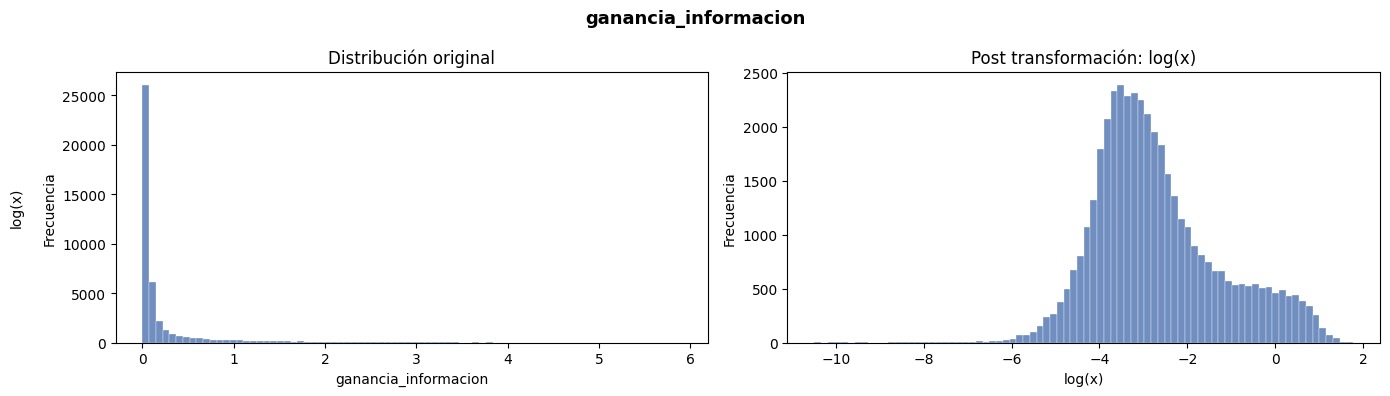
\includegraphics[width=\textwidth]{chapters/03_analisis_features/images/transf_ganancia_informacion.png}
    \caption{Distribución de la variable ganancia\_información transformada}
    \label{fig:transf_ganancia_informacion}
\end{figure}

La feature \feat{posterior} presenta un sesgo más pronunciado: prácticamente todos los valores se concentran en torno a cero, 
lo cual es consistente con su naturaleza. Se exploraron dos transformaciones: la transformación 
$\log(x)$ produce una distribución aproximadamente simétrica y unimodal, 
reduciendo efectivamente el sesgo original; la transformación logit produce 
un resultado distribucional similar.


\begin{figure}[H]
    \centering
    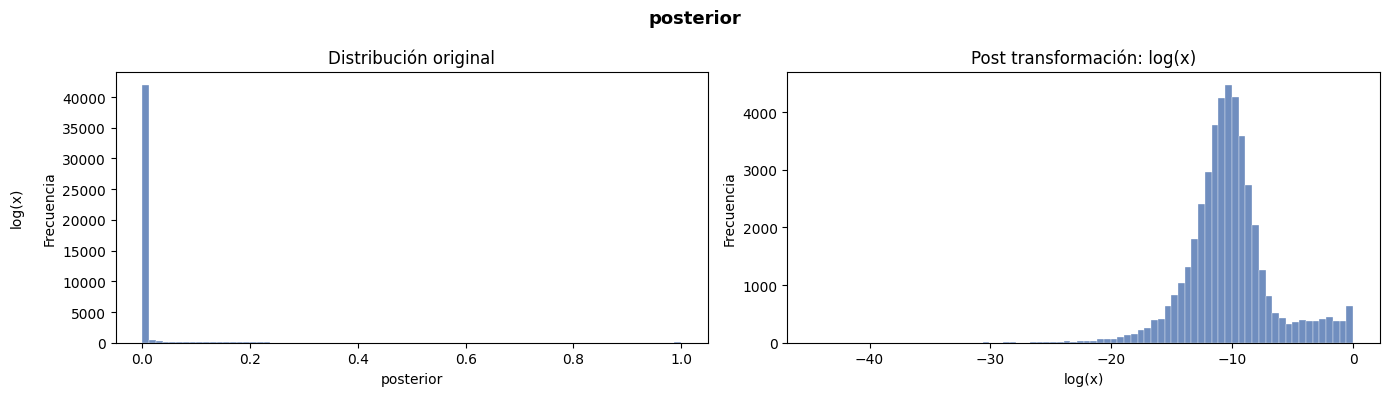
\includegraphics[width=\textwidth]{chapters/03_analisis_features/images/transf_posterior_log.png}
    \caption{Distribución de la variable posterior transformada}
    \label{fig:transf_posterior_log}
\end{figure}

\subsubsection{Transformaciones a features de Calidad de la decisión}

La feature \feat{gap\_entropia} presenta en su escala original una distribución 
sesgada a la derecha con cola extendida. La aplicación de $\log(x)$ mejora 
la simetría de la distribución, produciendo una forma aproximadamente unimodal, 
aunque persiste una leve asimetría en la cola derecha.

\begin{figure}[H]
    \centering
    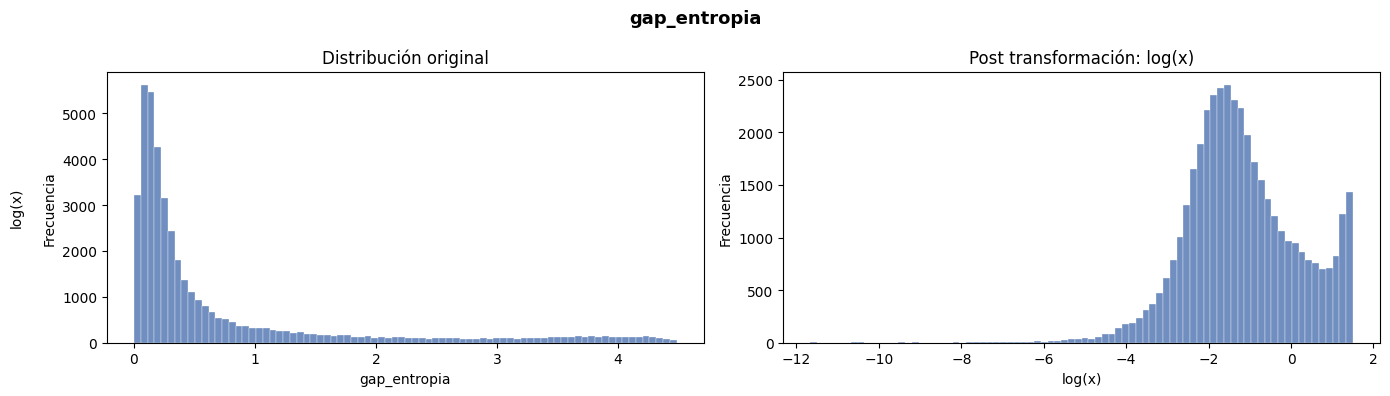
\includegraphics[width=\textwidth]{chapters/03_analisis_features/images/transf_gap_entropia.png}
    \caption{Distribución de la variable gap\_entropia transformada}
    \label{fig:transf_gap_entropia}
\end{figure}


La feature \feat{distancia\_grilla} presenta un comportamiento distinto al 
resto de las features analizadas. Su distribución original no corresponde 
a un caso clásico de sesgo a la derecha sino que exhibe una estructura 
multimodal con picos discretos, lo cual es esperable dado que esta feature 
toma valores enteros que representan distancias en celdas. La aplicación 
de $\log(x)$ no resuelve esta irregularidad: la distribución transformada 
mantiene la misma estructura discreta, dado que la transformación logarítmica 
preserva el orden y la separación entre valores enteros consecutivos.

\begin{figure}[H]
    \centering
    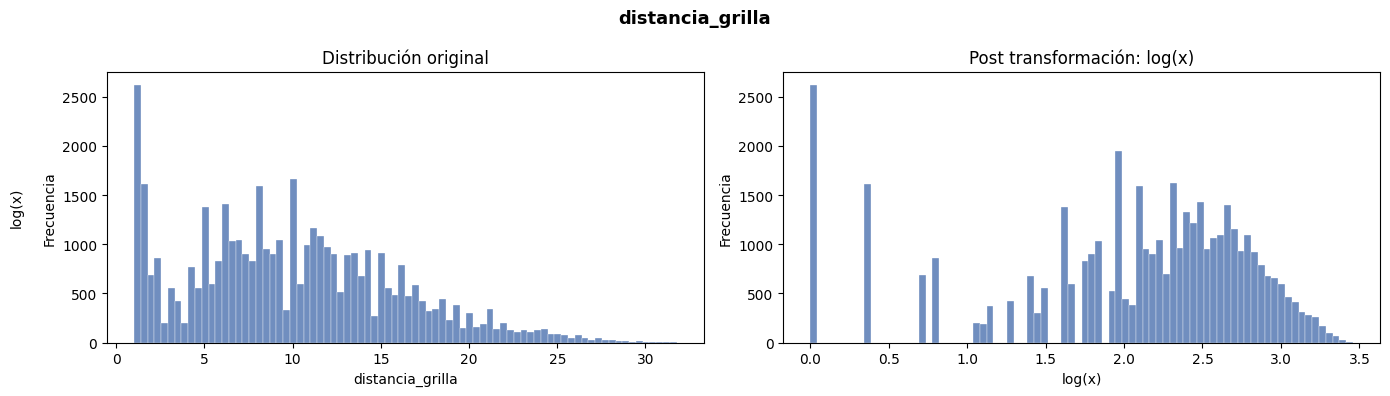
\includegraphics[width=\textwidth]{chapters/03_analisis_features/images/transf_distancia_grilla.png}
    \caption{Distribución de la variable distancia\_grilla transformada}
    \label{fig:transf_distancia_grilla}
\end{figure}

\subsubsection{Transformaciones a features de Competencia entre candidatos}

La feature \feat{competencia\_densidad} presenta en su escala original una 
distribución con sesgo extremo a la derecha y cola muy extendida. A diferencia 
de los casos anteriores, la aplicación de $\log(x)$ no resuelve el problema 
distribucional: la distribución transformada mantiene una estructura irregular 
dominada por pocos valores discretos, lo que sugiere que esta feature no se 
beneficia de una transformación logarítmica.

\begin{figure}[H]
    \centering
    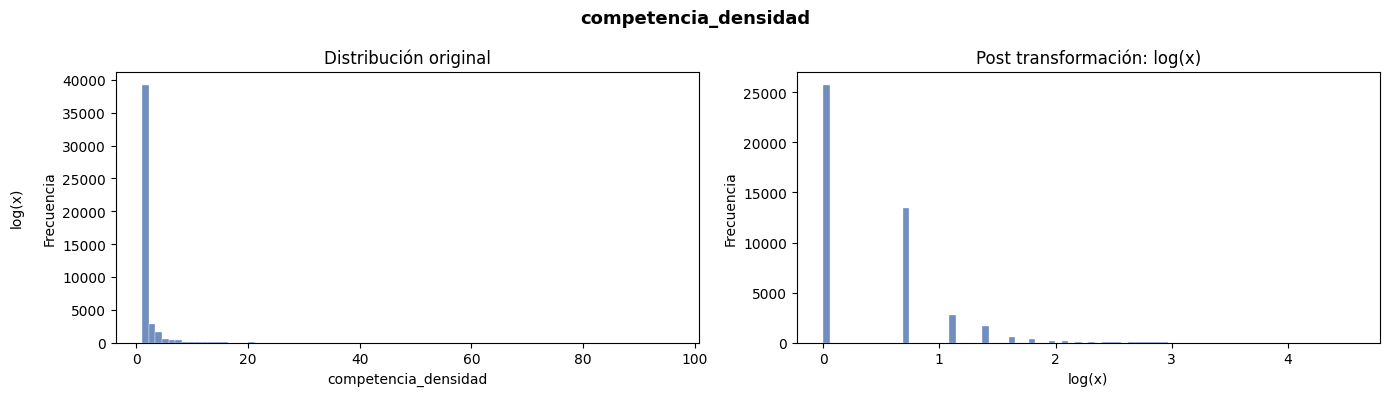
\includegraphics[width=\textwidth]{chapters/03_analisis_features/images/transf_competencia_densidad.png}
    \caption{Distribución de la variable distancia\_grilla transformada}
    \label{fig:transf_competencia_densidad}
\end{figure}

La feature \feat{competencia\_fp\_max} presenta también una distribución 
fuertemente sesgada a la derecha en su escala original. La aplicación de 
$\log(x)$ mejora considerablemente la distribución, produciendo una forma 
más simétrica, aunque persiste una leve asimetría a la izquierda y un pico 
aislado en el extremo derecho.

\begin{figure}[H]
    \centering
    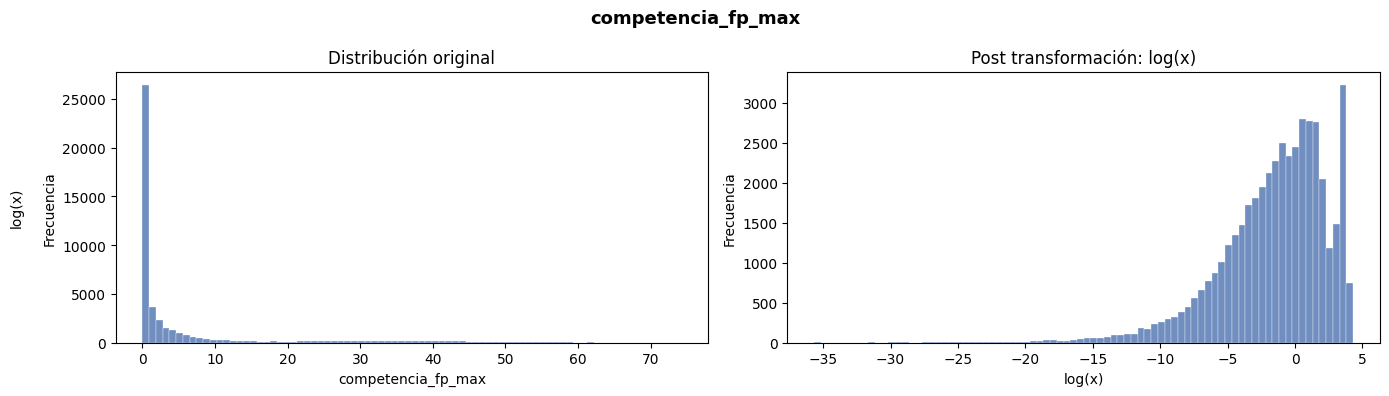
\includegraphics[width=\textwidth]{chapters/03_analisis_features/images/transf_competencia_fp_max.png}
    \caption{Distribución de la variable distancia\_grilla transformada}
    \label{fig:transf_competencia_fp_max}
\end{figure}